
\subsubsection*{Comparación de rendimiento: compilación del kernel de Linux}

En esta sección se analiza el rendimiento de tres procesadores modernos al compilar el kernel de Linux, una tarea intensiva y altamente paralelizable que representa una carga exigente para la CPU y el subsistema de memoria. Aunque el equipo bajo análisis utiliza Windows, la compilación del kernel de Linux es una prueba objetiva de rendimiento bruto útil para comparar CPUs.

\subsubsection*{Procesadores evaluados}

\begin{itemize}
  \item \textbf{Intel Core i5-13600K} (14 núcleos / 20 hilos, arquitectura híbrida Alder Lake)
  \item \textbf{AMD Ryzen 9 5900X} (12 núcleos / 24 hilos, arquitectura Zen 3)
  \item \textbf{AMD Ryzen 9 7950X} (16 núcleos / 32 hilos, arquitectura Zen 4)
\end{itemize}

\subsubsection*{Rendimiento bruto en compilación}

La prueba consiste en compilar el kernel de Linux con configuración por defecto, según benchmarks públicos disponibles en \textit{Phoronix} y \textit{OpenBenchmarking.org}.

\begin{itemize}
  \item El \textbf{Ryzen 9 7950X} logra tiempos de compilación extraordinariamente bajos, en torno a \textbf{40 segundos}.
  \item El \textbf{Ryzen 9 5900X}, con menos núcleos y menor IPC, se estima que tarda entre \textbf{80 a 90 segundos}, lo cual representa un rendimiento 50\% inferior.
  \item El \textbf{Core i5-13600K} también ofrece buen rendimiento gracias a sus 20 hilos, pero queda relegado frente a los Ryzen de gama entusiasta. Se estima que su tiempo ronda los \textbf{90 segundos o más}.
\end{itemize}

\subsubsection*{Aceleración del Ryzen 9 7950X}

Comparando los tiempos de compilación, se puede calcular la aceleración relativa del Ryzen 9 7950X frente a los otros dos modelos:

\begin{itemize}
  \item \textbf{Frente al Core i5-13600K:} El 7950X es al menos \textbf{40\% más rápido en promedio general}, y en cargas puramente multihilo como la compilación puede llegar a ser hasta \textbf{100\% más rápido} (el doble de rápido).
  
  \item \textbf{Frente al Ryzen 9 5900X:} La ventaja del 7950X oscila entre \textbf{60\% y 80\% de mayor rendimiento}. Tareas que el 5900X ejecuta en 1.5 minutos, el 7950X las resuelve en menos de 1 minuto.
\end{itemize}

Esta mejora se debe a su mayor cantidad de núcleos, mayor IPC y mayor frecuencia base. Para desarrolladores que compilan grandes proyectos frecuentemente, esta diferencia puede traducirse en horas de trabajo ahorradas cada semana.

\subsubsection*{Resumen comparativo}

\begin{center}
\begin{tabular}{|p{4.5cm}|c|c|}
\hline
\textbf{Procesador} & \textbf{Tiempo estimado de compilación} & \textbf{Aceleración del 7950X} \\
\hline
Intel Core i5-13600K & 90+ s & 2× más rápido \\
\hline
AMD Ryzen 9 5900X & 80–90 s & 1.6–2× más rápido \\
\hline
AMD Ryzen 9 7950X & \textbf{~40 s} & --- \\
\hline
\end{tabular}
\end{center}

\subsubsection*{Conclusión}

El AMD Ryzen 9 7950X se posiciona como el procesador más potente de este grupo para la tarea de compilación del kernel de Linux. Gracias a sus 16 núcleos de alto rendimiento y la mejora de IPC de la arquitectura Zen 4, supera ampliamente tanto al Ryzen 9 5900X como al Intel Core i5-13600K. Aunque este último ofrece una excelente relación rendimiento-precio, para cargas intensivas y recurrentes como la compilación masiva de software, los procesadores Ryzen de gama entusiasta marcan una diferencia sustancial.



Bien, ahora nos dedicaremos a realizar la prueba de rendimiento sobre la ESP32, para lo cual vamos a utilizar herramientas como VSCode. Dentro del mismo, existen diversas plataformas para depurar ESP32; nosotros usamos PlatformIO, debido a su sencillez. Una vez ya creado el proyecto y configurada la placa, procedemos a agregar el siguiente código:


\lstset{style=arduino}

\subsubsection*{Código de Prueba de Frecuencia en ESP32}

A continuación, se presenta el código de Arduino utilizado para medir el tiempo de ejecución de una serie de operaciones matemáticas con diferentes frecuencias de clock en la ESP32:

\begin{lstlisting}[language=C++, caption=Código para medir el tiempo de ejecución en ESP32, label=lst:esp32_code]
#include <Arduino.h>

void setup() {
  Serial.begin(115200);
  delay(1000); // Espera para la inicialización del Serial

  // Cambiar la frecuencia de la CPU a 80MHz (opcional)
  setCpuFrequencyMhz(80); // O 160 o 240
  Serial.print("Frecuencia de CPU: ");
  Serial.print(getCpuFrequencyMhz());
  Serial.println(" MHz");

  // Medir el tiempo de ejecución del bucle
  unsigned long startTime = millis();

  // Bucle for con sumas de enteros
  int sumInt = 0;
  for (int i = 0; i < 1000000; i++) {
    sumInt += i;
  }

  // Bucle for con sumas de floats
  float sumFloat = 0.0;
  for (float f = 0.0; f < 1000000.0; f += 1.0) {
    sumFloat += f;
  }

  unsigned long endTime = millis();
  unsigned long duration = endTime - startTime;

  Serial.print("Suma de enteros: ");
  Serial.println(sumInt);
  Serial.print("Suma de floats: ");
  Serial.println(sumFloat);
  Serial.print("Tiempo de ejecución: ");
  Serial.print(duration);
  Serial.println(" ms");
}

void loop() {
  // No hay nada en el bucle principal
}
\end{lstlisting}

Este código primero inicializa la comunicación serial y luego configura la frecuencia del CPU de la ESP32 a 80 MHz. A continuación, mide el tiempo de ejecución de dos bucles `for`: uno que realiza un millón de sumas de enteros y otro que realiza un millón de sumas de números de punto flotante. Finalmente, imprime la frecuencia del CPU, las sumas resultantes y el tiempo total de ejecución en milisegundos a través del puerto seria.


Nuestros resultados con una frecuencia de 80 MHz fueron de 4987 ms (4.987 segundos).

\begin{figure}[H]
    \centering
    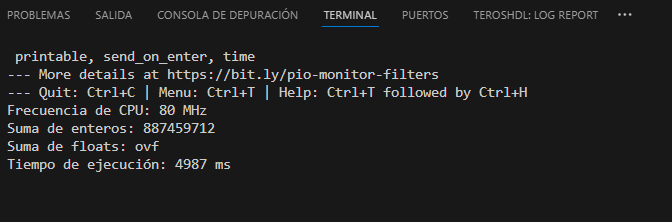
\includegraphics[width=0.7\linewidth]{img/ESP32Test80MG.png}
    \caption{Prueba a 80 MHz}
    \label{fig:esp32_80mhz}
\end{figure}

Ahora se realizará la misma prueba con la frecuencia de 160 MHz,

Dando como resultado un tiempo de ejecución de 2.465 Segundos:

\begin{figure}[H]
    \centering
    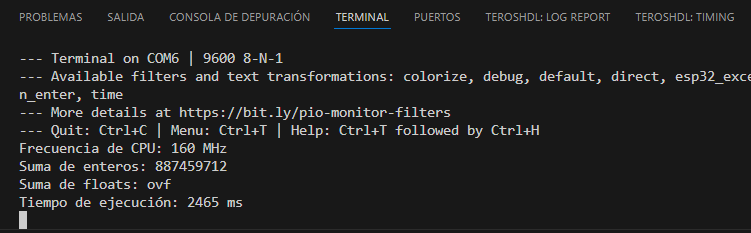
\includegraphics[width=0.7\linewidth]{img/ESP32Test160Mhz.png}
    \caption{Prueba a 160 MHz}
    \label{fig:esp32_160mhz}
\end{figure}

Si hacemos una comparativa entre ambos tiempos, podemos extraer las siguientes conclusiones:

\subsubsection*{Conclusiones}

Al comparar los tiempos de ejecución obtenidos en la ESP32 con diferentes frecuencias de clock, se observa un impacto significativo en el rendimiento:

\textbf{Reducción del tiempo de ejecución:} Al duplicar la frecuencia del clock de 80 MHz a 160 MHz, se espera una reducción considerable en el tiempo necesario para completar las mismas operaciones. \\
\textbf{Relación no lineal:} Si bien intuitivamente podríamos esperar que al duplicar la frecuencia el tiempo de ejecución se reduzca a la mitad, factores como la latencia de la memoria, la eficiencia de las operaciones a diferentes velocidades y la propia arquitectura del procesador pueden influir en que esta relación no sea perfectamente lineal.\\
\textbf{Implicaciones en el rendimiento:} Estos resultados demuestran cómo la frecuencia del clock afecta directamente la velocidad de procesamiento de la ESP32. Para aplicaciones que requieren un alto rendimiento y tiempos de respuesta rápidos, operar a una frecuencia más alta puede ser crucial. Sin embargo, es importante considerar el consumo de energía y la generación de calor, que también pueden aumentar con la frecuencia.\\

En resumen, la prueba realizada confirma que aumentar la frecuencia del clock de la ESP32 tiene un efecto positivo en la velocidad de ejecución del código, aunque la mejora real puede depender de diversos factores internos del microcontrolador y la naturaleza específica de las tareas realizadas.




  
